% \title{Wall Calendar version of CD calendars}

%%% The calendars are printed 2-up to fit CD jewel cases,
%%% or 4-up to fit 3" floppy disk jewel cases. OR, now a
%%% full-blown "giant" version that prints full-page!
%%%
%%% Localisation possible with languages supported by
%%% babel/translator/datetime2.
%%% Tested with british, spanish, french, ngerman,
%%% italian, portuges, polish, croatian, greek, bahasai,
%%% bahasam.
%%%
%%% bahasai (Indonesian) works with the following new or modified files in this project:
%%% - translator-language-mappings.tex
%%% - translator-months-dictionary-Indonesian.dict
%%% - datetime2-bahasai.ldf
%%%
%%% bahasam (Bahasa Malaysia) works with the following new or
%%% modified files in this project:
%%% - translator-language-mappings.tex
%%% - translator-months-dictionary-Malaysian.dict
%%% - datetime2-bahasam.ldf
%%%
%%% (Use lualatex for french. If using pdflatex for greek,
%%% Remember to load LGR,T1 for fontenc.)
%%%
%%% NOTE: If you get an error when you change the language,
%%% click on the "compile from scratch" option in the error
%%% message window.
\documentclass[20pt,british,giant]{cdcalendar}
%%% Use the sundayweek option for weeks to start on Sundays.
% \documentclass[20pt,british,sundayweek,giant]{cdcalendar}

%% If using pdfLaTeX %%%%%%%%%%
\usepackage[utf8]{inputenc}
\usepackage[T1]{fontenc}

% Using Gentium and Open Sans
\usepackage{gentium}
\usepackage[defaultsans,osfigures,scale=0.94]{opensans}
%% End pdfLaTeX-related font settings %%%%%%%%


% %% Compile with luaLaTeX if using fontspec
% \usepackage{fontspec}
% \setmainfont{Gentium}
% \setsansfont[BoldItalicFont=Fira Sans Italic,BoldFont=Fira Sans]{Fira Sans Light}
% %% End luaLaTeX-related font settings %%%%%%%%


\usepackage{graphicx}
\usepackage{wallpaper}
\graphicspath{{img/}}
% Default values -- change if needed
% \setlength{\CalPageMargin}{1cm}
% \setlength{\EventLineWidth}{6in}
% \geometry{a4paper}

\begin{document}

%%%%%%
% Cover
%%%%%%
\coverBgColor{RoyalBlue!40!black}
\coverImage{LuncheonoftheBoatingParty}
\coverTitle[font=\fontsize{48pt}{50pt}\sffamily\bfseries,text=white,text width=\linewidth,align=flush right]{Coventry City Council 2015/16 School Year}

\makeCover

%%%% Remove this page if you don't need it --
%%%% just to show the actual output for the jewel case
%%%% calendars
% {\centering
% 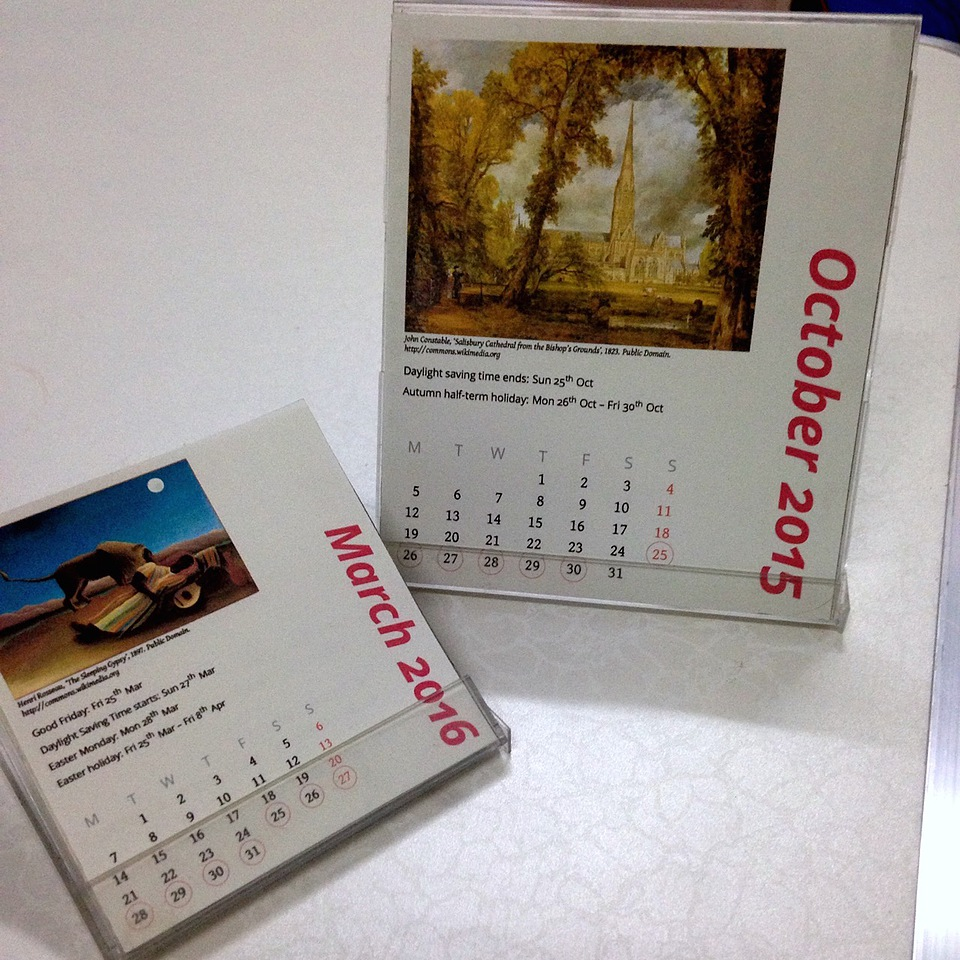
\includegraphics[width=\textwidth]{actual}
% \par}

% Here are the actual printed calendars. The smaller calendar (9cm $\times$ 9.5cm) fits floppy disk jewel cases; while the bigger one (11.7cm $\times$ 13.65cm) fits CD jewel cases.

% \clearpage
%%%%


%%%%%%
% Some settings for the monthly calendars
%%%%%%
\dayHeadingStyle{font=\sffamily\color{gray!90}}
\sundayColor{red}
\monthTitleStyle{font={\fontsize{40pt}{42pt}\bfseries\sffamily\itshape\selectfont}, red!50!RedViolet}
\eventStyle{\scriptsize\sffamily}

% Remove this line if you feel the background pattern is too annoying
\TileWallPaper{.5\paperwidth}{.5\paperheight}{ricepaper_v3}

% You may find the gap between illustrations and events too wide
% Use this length to lessen it
\setlength{\lessIllusSkip}{1ex}


%%%%%%
% September 2015
%%%%%%
\illustration[Vincent van Gogh, `The Starry Night', 1889. Public Domain. \url{http://commons.wikimedia.org}]{\linewidth}{StarryNight}

\monthCalendar{2015}{09}

%%% events must be given AFTER \monthCalendar
%%% Currently you must give events on the same page
%%% as the monthly calendar.

%% This is an one-day event
\event{2015-09-02}{Autumn school term starts}

\clearpage


%%%%%%
% Oct 2015
%%%%%%
\illustration[John Constable, `Salisbury Cathedral from the Bishop's Grounds', 1823. Public Domain. \url{http://commons.wikimedia.org}]{\linewidth}{SalisburyCathedral}

\monthCalendar{2015}{10}

\event{2015-10-25}{Daylight saving time ends}

%% This is a 5-day event starting Oct 26th
\event[5]{2015-10-26}{Autumn half-term holiday}

%% You could also write
%\event[2015-10-30]{2015-10-26}{Autumn half-term holiday}

\clearpage

%%%%%%
% Nov 2015
%%%%%%
\illustration[Jin Nong, `Flower', 1754. Public Domain. \url{http://commons.wikimedia.org}]{\linewidth}{Flower_JinNong}

\monthCalendar{2015}{11}

\clearpage


%%%%%%
% Dec 2015
%%%%%%
\illustration[Hendrick Avercamp, `Winter Landscape with Ice Skaters', c.~1608. Public Domain. \url{http://commons.wikimedia.org}]{\linewidth}{WinterLandscape}

\monthCalendar{2015}{12}

\event{2015-12-18}{Last day of Autumn term}

\event{2015-12-25}{Christmas Day}

\event{2015-12-28}{Boxing Day (substitute)}

\clearpage

%%%%%%
% January 2016
%%%%%%
\illustration[Auguste Renoir, `Oarsmen at Chatou', 1879. Open Access. \url{https://images.nga.gov}]%
{\linewidth}{A17050}

\monthCalendar{2016}{01}

\event{2016-01-01}{New Year's Day}

\event{2016-01-04}{Spring term starts}

\clearpage

%%%%%%
% February 2016
%%%%%%
\illustration[Cariani, `Concert', c.~1518--1520. Open Access. \url{https://images.nga.gov}]%
{\linewidth}{A10623}

\monthCalendar{2016}{02}

%% This is a 5-day event starting on Feb 15
\event[5]{2016-02-15}{Spring half-term holiday}

\clearpage

%%%%%%
% March 2016
%%%%%%
\illustration[Henri Rosseau, `The Sleeping Gypsy', 1897. Public Domain. \url{http://commons.wikimedia.org}]{\linewidth}{SleepingGypsy}

\monthCalendar{2016}{03}

\event{2016-03-25}{Good Friday}

\event{2016-03-27}{Daylight Saving Time starts}

\event{2016-03-28}{Easter Monday}


%% Note if a multi-day event extends to the next month,
%% you'll have to list it again in the next month.
%% This event starts on March 25 and ends on April 8.
\event[2016-04-08]{2016-03-25}{Easter holiday}

\clearpage


%%%%%%
% April 2016
%%%%%%
\illustration[Katsushika Hokusai, `The Great Wave of Kanagawa', 1823--1829. Public Domain. \url{http://commons.wikimedia.org}]{\linewidth}{Tsunami}

\monthCalendar{2016}{04}

\event[2016-04-08]{2016-03-25}{Easter holiday}

\clearpage

%%%%%%
% May 2016
%%%%%%
\illustration[John Everett Millais, `Ophelia', circa 1851. Public Domain. \url{http://commons.wikimedia.org}]{\linewidth}{Ophelia}

\monthCalendar{2016}{05}

\event{2016-05-02}{Early May bank holiday}

\event{2016-05-30}{Spring Bank Holiday}

\event[5]{2016-05-30}{Summer half-term holiday}

\clearpage

%%%%%%
% June 2015
%%%%%%
% {\huge\color{BurntOrange} Deep summer is when laziness finds respectability.\par}
% {\raggedleft -- Sam Keen\par}
\illustration[J.M.W.~Turner, `The Fighting Temeraire tugged to her last berth to be broken up', 1839. Public Domain. \url{http://commons.wikimedia.org}]{\linewidth}{FightingTemeraire}

\monthCalendar{2016}{06}

\event[5]{2016-05-30}{Summer half-term holiday}

\clearpage

%%%%%%
% July 2016
%%%%%%
\illustration[Édouard Manet, `A Bar at the Folies-Bergère', 1881 -- 1882. Public Domain. \url{http://commons.wikimedia.org}]{\linewidth}{BarAtTheFoliesBergere}

\monthCalendar{2016}{07}

\event{2016-07-21}{Summer holiday begins}
\clearpage

%%%%%%
% August 2016
%%%%%%
\illustration[Georges Seurat, `A Sunday Afternoon on the Island of La Grande Jatte', 1884 -- 1886. Public Domain. \url{http://commons.wikimedia.org}]{\linewidth}{SundayOnLaGrandeJatte}

\monthCalendar{2016}{08}

\event{2016-08-29}{Summer bank holiday}
\event{2016-09-06}{New school year begins}

\clearpage

\end{document}
